
An interesting behaviour of the neutrinos is that they change flavour
changes when they propagate. The simplest way to explain this
phenomenon is via neutrino oscillations, which leads to the conclusion
that they have mass. This behaviour is not unique in particle physics
as it has been observed for kaons and B-mesons. The oscillations of
neutrinos had been postulated a long time before by Pontecorvo in
1958~\cite{Pontecorvo1958} and later by Maki, Nakagawa and
Sakata~\cite{Maki:1962mu}. The evidences that neutrinos oscillate is
fairly recent; it dates from 1998 with the Super-Kamiokande
detector~\cite{SK1998}. The evidence was confirmed later by the
\Gls{SNO} experiment in 2002~\cite{SNO2002}. The spokespersons of
these experiments were awarded the Nobel Prize of physics for the
discovery of neutrino oscillation and the implication that had on
neutrino mass~\cite{nobelprize}.

This section introduces an approximated mathematical formalism to the
phenomenon of neutrino oscillations.  The main approximation is that
the formalism is not Lorentz invariant. To have a Lorentz invariant
equation, a full Quantum Field Theory (QFT) approach is required,
which is beyond the scope of this introduction~\cite{Akhmedov2010}. In
broad terms, it consists of calculating amplitudes of Feynman diagrams
such as the one in Figure~\ref{fig:neutrinooscillationdiag}, where the
neutrino is considered as a propagator.

\begin{figure}[ht]
  \vspace{1cm}
  \center
  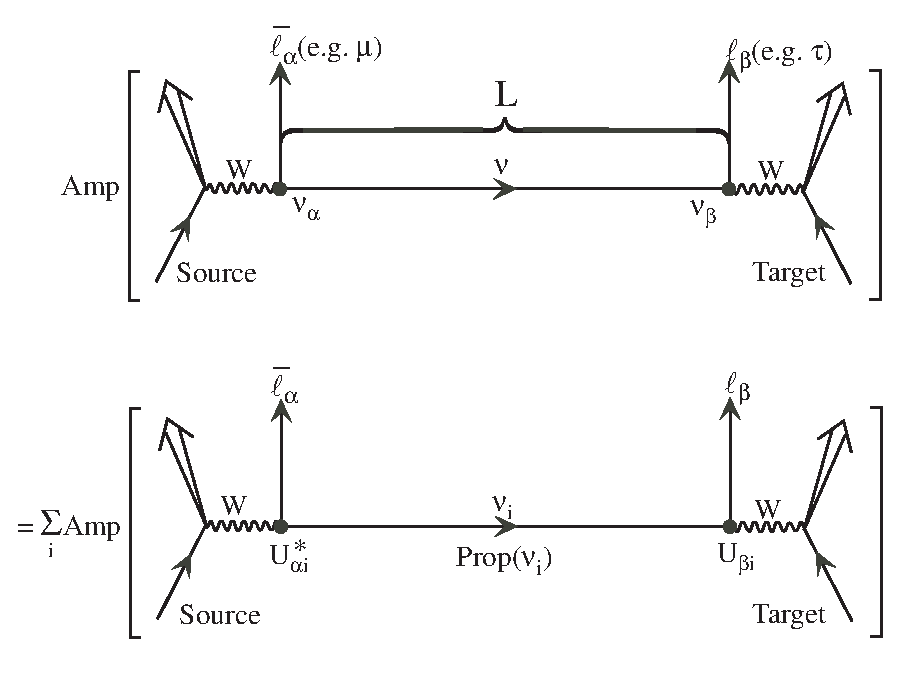
\includegraphics[width=0.98\textwidth]{images/Intro/SLAC_Fig1.eps}
  \caption[Neutrino flavour change (oscillation) in vacuum]{Neutrino
    flavour change (oscillation) in vacuum. “Amp” denotes an
    amplitude. Taken from~\cite{Kayser:2005cd}.}
  \label{fig:neutrinooscillationdiag}
\end{figure}

The oscillation relies on the hypothesis that the neutrino mass and
flavour states have the same momentum. These equations are developed
in the case of relativistic neutrino, which is true for all detectable
neutrinos\footnotemark.  It is worth noting that although this
derivation lacks physical motivation and robustness compared to a full
rigorous QFT approach, it leads to the exact same answer.

\footnotetext{The neutrinos have a mass smaller than few
  eVs~\cite{Troitsk}, and detectable neutrinos have energy greater
  than few hundreds of keVs~\cite{GALLEX1999}}

To show that neutrinos oscillate, one can start with the common
expressions of the flavours state as a function of the mass state via
the \Gls{PMNS} (Pontecorvo-Maki-Nakagawa-Sakata)
matrix~\cite{Pontecorvo:1967fh,Pontecorvo:1957cp,Bilenky:1978nj,Maki:1962mu}:

\begin{align}
  \colvec{
    \nu_e    \\
    \nu_\mu  \\
    \nu_\tau
  }
  &= \colvec{
    U_{e1} & U_{e2} & U_{e3}\\
  U_{\mu1} &U_{\mu2}  &U_{\mu3}\\
  U_{\tau1} &U_{\tau2}  &U_{\tau3}
                          }
  \colvec{
    \nu_1 \\
    \nu_2 \\
    \nu_3
  } \label{eq:pmnsugly}\\
  &=
  \colvec{
    1 & 0       & 0     \\
    0 & c_{23}  & s_{23} \\
    0 & -s_{23} & c_{23}
  }
  \colvec{
    c_{13}               & 0 & s_{13}e^{-i \delta_{\text{CP}}} \\
    0                    & 1 & 0                      \\
    -s_{13}e^{i \delta_{\text{CP}}} & 0 & c_{13}
  }
  \colvec{
    c_{12}  & s_{12} & 0 \\
    -s_{12} & c_{12} & 0 \\
    0      & 0      & 1
  }
  \colvec{
    1 & & \\
    & e^{-i\frac{\alpha_{21}}{2}} &\\
    & & e^{-i\frac{\alpha_{31}}{2}}\\
  }
  \colvec{
    \nu_1 \\
    \nu_2 \\
    \nu_3
  }                ,
  \label{eq:pmns}
\end{align}
which quantifies the massive content of the flavour neutrino $\nu_e$,
$\nu_\mu$ and $\nu_\tau$ according to their mass eigenstates $\nu_1$,
$\nu_2$ and $\nu_3$. Each $c_{ij}$ and $s_{ij}$ reads
$\cos\left(\theta_{ij}\right)$ and $\sin\left(\theta_{ij}\right)$
respectively, where $\theta_{ij}$ are the mixing
angles. $\delta_{\text{CP}}$ ($\alpha_{21}$, $\alpha_{31}$) are the
Dirac (Majorana) phases indicating \Gls{CP} (Charge Parity) violation.
Equation~\ref{eq:pmnsugly} is the general form for the \Gls{PMNS}
matrix, and Equation~\ref{eq:pmns} is a more elegant way to
parametrise it. Note that, in the absence of oscillations of the
active neutrinos to sterile neutrinos. Since there is no experimental
observations of oscillations to sterile neutrinos, these matrices
considered are unitary.

With Equation~\ref{eq:pmns}, one factorises in ``sectors'' the
oscillations according to the type of neutrino oscillation which are
observed. Hence, the first matrix relates to the ``atmospheric
sector,'' which, at first order, describes the oscillation of
$\nu_\mu\rightarrow\nu_\tau$. The third matrix describes the ``solar
sector'' that quantifies the oscillation of
$\nu_e\rightarrow\nu_\mu$. Finally, the second matrix is the ``cross
mixing'' matrix, which depends on the Dirac phase in its off-diagonal
terms. This phase encloses the difference in the oscillatory behaviour
between neutrinos and anti-neutrinos.

The calculation which leads to the conclusion that the neutrino of a
certain flavour oscillates to another during its propagation is now
quickly developed.

Supposing a neutrino of a defined flavour is created in space-time,
one can write:
\begin{equation}
  \label{eq:superposition}
  \ket{\nu_\alpha} = \sum_{k}U^{*}_{\alpha k} \ket{\nu_k} (\alpha = e,\mu,\tau),
\end{equation}
where \(\nu_\alpha\) are the flavour eigenstates and \(\nu_k\) are the
mass eigenstates. This is just another way of writing
Equation~\ref{eq:pmnsugly}. The term \(U^{*}_{\alpha k}\) is an
element of the mixing matrix. Next, the neutrino mass states are
orthogonal, so this leads to
\begin{equation}
  \braket{\nu_k|\nu_j}=\delta_{kj}
\end{equation}
and similarly for the flavour states:
\begin{equation}
  \braket{\nu_\alpha|\nu_\beta}=\delta_{\alpha\beta}.
\end{equation}

The massive states $\ket{\nu_k}$ are eigenstates of the Hamiltonian
operator $\mathcal{H}$:
\begin{equation}
  \mathcal{H}\ket{\nu_k}=E_k\ket{\nu_k},
\end{equation}
and, solving this equation, one reaches:
\begin{equation}
  \label{eq:schrodinger}
  \ket{\nu_k(t)} = \exp (-iE_k t)\ket{\nu_k}.
\end{equation}

Consider now a neutrino of flavour $\alpha$, that was created at
$t=0$, $\ket{\nu_\alpha(t=0)}$. This neutrino propagates in
space-time, using Equation~\ref{eq:schrodinger} and
\ref{eq:superposition}, one can write:
\begin{equation}
  \label{eq:prop} \ket{\nu_\alpha(t)} = \sum_k U_{\alpha
    k} \exp (-iE_kt)\ket{\nu_k},
\end{equation} for which, if $t=0$, $\ket{\nu_\alpha(t=0)} =
\ket{\nu_\alpha}$.

Note that it is possible to invert Equation~\ref{eq:superposition}:
\begin{equation}
  \label{eq:superpositioninvert} \ket{\nu_k}=\sum_\alpha U_{\alpha
k}\ket{\nu_\alpha},
\end{equation}
and that can be inserted into Equation~\ref{eq:prop}:
\begin{equation}
\ket{\nu_{\alpha}(t)}=\sum_{\beta=e,\mu,\tau}\left(\sum_{k}U^*_{\alpha
k}\exp\left(-iE_kt\right)U_{\beta k}\right)\ket{\nu_\beta}.
\end{equation}

Hence, for an arbitrary time $t$, one can see that the
$\ket{\nu_\alpha(t)}$ is a superposition of the states
$\ket{\nu_\beta}$. This means the neutrino created at $t=0$ is now a
composite state of the different flavour neutrinos. Consider now the
amplitude of the oscillation process
$\nu_\alpha\rightarrow \nu_\beta$,
$\mathcal{A}_{\nu_\alpha\rightarrow\nu_\beta}$:
\begin{align}
  \mathcal{A}_{\nu_\alpha\rightarrow\nu_\beta}(t) &= \braket{\nu_\beta|\nu_\alpha(t)}\\
                                                  &=\sum_kU^*_{\alpha k}U_{\beta k}\exp(-iE_kt),
\end{align}
which can be squared to get the probability of oscillation:
\begin{align}
  \mathcal{P}_{\nu_\alpha\rightarrow\nu_\beta} &= \left|\mathcal{A}_{\nu_\alpha\rightarrow\nu_\beta}\right|^2 \nonumber \\
                             &=\sum_{k,j}U^*_{\alpha k}U_{\beta k}U_{\alpha j}U^*_{\beta j}\exp\left(-i(E_k-E_j)t\right). \label{eq:prob}
\end{align}

Further simplification can be made to reach a simple equation. First,
the energy for any particle is given by:
\begin{equation}
  E_k=\sqrt{m_k^2+\vec{p}^{\,2}}
\end{equation}
and that can be simplified with a simple Taylor expansion for the case of
large momentum (i.e. relativistic particle):
\begin{equation}
  E_k\simeq |p|+\frac{m_k^2}{2|p|},
\end{equation}
which can be reinserted in the exponential term of Equation~(\ref{eq:prob}):
\begin{equation}
  E_k-E_j\simeq \frac{m_k^2-m_j^2}{2|p|}.
\end{equation}

In this equation, it is assumed that the momentum of the mass states
during the creation of the neutrino is the same, $p$. One can then
define $\Delta m_{kj}^2 = m_k^2-m_j^2$, and replace $|p|$ by $E$ since
the neutrinos are ultra-relativistic. Substituing everything in
Equation~(\ref{eq:prob}) leads to:
\begin{equation}
  \mathcal{P}_{\nu_\alpha\rightarrow\nu_\beta}=\sum_{k,j}U^*_{\alpha k}U_{\beta k}U_{\alpha j}U^*_{\beta j}\exp\left(-i(\Delta m_{kj}^2)t/(2E)\right).
\end{equation}

One further simplification comes from the fact that the neutrino are
propagating at almost the speed of light, $c$, which equates 1 in
natural units. So $t=L$, where $L$ is the distance of propagation of
the neutrino:

\begin{equation}
  \mathcal{P}_{\nu_\alpha\rightarrow\nu_\beta}=\sum_{k,j}U^*_{\alpha k}U_{\beta k}U_{\alpha j}U^*_{\beta j}\exp\left(-i(\Delta m_{kj}^2)L/(2E)\right).
\end{equation}

Finally, this probability can be simplified to:
\begin{align}
  \label{eq:oscilprob}
  \mathcal{P}_{\nu_\alpha\rightarrow\nu_\beta} =\delta_{\alpha\beta}&-4\sum_{k>j}\mathcal{Re}\left[U^*_{\alpha k}U_{\beta k}U_{\alpha j}U^*_{\beta j} \right]\sin^2\left(\frac{\Delta m^2_{kj}L}{4E}\right)  \nonumber \\
                                                                    &+2\sum_{k>j}\mathcal{Im}\left[U^*_{\alpha k}U_{\beta k}U_{\alpha j}U^*_{\beta j}\right]\sin\left(\frac{\Delta m_{kj}^2L}{2E}\right).
\end{align}

Note that the oscillation probability depends on terms of the form
$U^*_{\alpha k}U_{\beta k}U_{\alpha j}U^*_{\beta j}$ for which the
Majorana phases systematically cancel, which is why neutrino
oscillation experiments cannot detect these phases. These Majorana
phases can be determined via the detection of neutrinoless double beta
decay processes~\cite{Furry1939}.

In the case of \Gls{TK}, which measures electron neutrinos in a muon
neutrino beam of~600~MeV at a distance of 295~km, the oscillation
probability, Equation~\ref{eq:oscilprob},
becomes~\cite{Cervera:2000kp}:

\begin{align}
  \label{eq:numu-numu}
  \mathcal{P}_{\nu_\mu\rightarrow\nu_\mu} &= \mathcal{P}_{\bar{\nu}_\mu\rightarrow\bar{\nu}_\mu}\\
                                          &\simeq 1 - 4\cos^2\theta_{13}\sin^2\theta_{23}\left[1-\cos^2\theta_{13}\sin^2\theta_{23}\right]\sin^2\left(\frac{\Delta m^2_{32}L}{4E}\right), \nonumber
\end{align}
for the muon neutrino survival probability and
\begin{align}
  \mathcal{P}(\bbar{\nu}_{\mu} \rightarrow \bbar{\nu}_e) &\simeq \sin^2\theta_{23} \sin^22\theta_{13} \sin^2\left(\frac{\Delta m^2_{31} L}{4E}\right) \nonumber \\
                                                         &\bplus{-} \text{~}\frac{\sin2\theta_{12} \sin2\theta_{23}}{2\sin\theta_{13}} \sin\left(\frac{\Delta m^2_{21} L}{4E}\right) \times \sin^22\theta_{13} \sin^2\left(\frac{\Delta m^2_{31} L}{4E}\right) \sin\delta_{CP},
  \label{eq:numu-nue}
\end{align}
for the electron (anti-) neutrino appearance
probability. Figure~\ref{fig:oscillationprob} shows these oscillation
probabilities in the case of \Gls{TK} for typical values of the
parameters measured at \Gls{TK} (and reported in
Table~\ref{tab:oscillation_parameters}).

\begin{figure}[ht]
  \center
  \includegraphics[width=0.8\textwidth]{images/Intro/Oscillation.pdf}
  \caption[Neutrino oscillation probability at T2K]{Neutrino
    oscillation probability at \Gls{TK}, for normal ordering,
    $\delta_{CP}=\pi/2$ and using the values given in
    Table~\ref{tab:oscillation_parameters}. Produced with
    Prob3++~\cite{prob3pp}.}
  \label{fig:oscillationprob}
\end{figure}


The Dirac phase, $\delta_{CP}$, is the last of parameter of the matrix
that remains to be measured. All the \Gls{PMNS} angles value are given
in Table~\ref{tab:oscillation_parameters}, along with the differences
of mass squared, $|\Delta m^2_{jk}|$. Note that this table
differentiates the normal and inverted ordering: this is because
neutrino oscillations are yet insensitive to the sign of the mass of
the atmospheric mass squared splitting. This can be seen in both
Equation~(\ref{eq:numu-numu}) and (\ref{eq:numu-nue}): the first,
dominant, term always appears squared
($\sin^2\left(\frac{\Delta m^2_{32}L}{4E}\right)$, for example), hence
experiments still do not have access to signs of $\Delta m_{31}$ and
$\Delta m_{32}$. Both hypotheses for the mass ordering are illustrated
in Figure~\ref{fig:ordering}. In the normal ordering case (left of the
figure), the mass states are ordered by increasing order:
$m_{\nu_1}<m_{\nu_2}<m_{\nu_3}$; in the inverted case (right of the
figure), the mass states are ordered in a different way:
$m_{\nu_3}<m_{\nu_1}<m_{\nu_2}$.

\begin{figure}[ht]
  \center
  \includegraphics[width=0.8\textwidth]{images/Intro/mass-hierarchy.png}
  \caption[Possible neutrino mass ordering]{Possible neutrino mass
    ordering. \textbf{\textit{Left:}} Normal ordering
    case. \textbf{\textit{Right:}} Inverted ordering case. Reproduced
    from~\cite{massordering}}
  \label{fig:ordering}
\end{figure}





\begin{table}[ht!]
  \begin{adjustbox}{center}
    \begin{tabular}{llll}
      \toprule
      Parameter & Ordering & Best fit value& $3 \sigma$ range  \\
      \midrule%---------------------------------------------------------------------
      $\Delta m_{21}^2/10^{-5}~\mathrm{eV}^2 $ & NO, IO, Any & 7.37 & 6.93 -- 7.96 \\
      \midrule%---------------------------------------------------------------------
      $\sin^2 \theta_{12}/10^{-1}$        & NO, IO, Any & 2.97 & 2.50 -- 3.54 \\
      \midrule%---------------------------------------------------------------------
      $|\Delta m^2|/10^{-3}~\mathrm{eV}^2 $ & NO  & 2.525 & 2.411 -- 2.646 \\
                & IO  & 2.505 & 2.390 -- 2.624 \\
                & Any & 2.525 & 2.411 -- 2.646 \\
      \midrule%---------------------------------------------------------------------
      $\sin^2 \theta_{13}/10^{-2}$ & NO  & 2.15 & 1.90 -- 2.40 \\
                & IO  & 2.16 & 1.90 -- 2.42 \\
                & Any & 2.15 & 1.90 -- 2.40 \\
      \midrule%---------------------------------------------------------------------
      $\sin^2 \theta_{23}/10^{-1}$ & NO  & 4.25 & 3.81 -- 6.15 \\
                & IO  & 5.89 & 3.84 -- 6.36 \\
                & Any & 4.25 & 3.81 -- 6.26 \\
      \midrule%---------------------------------------------------------------------
      $\delta_{\text{CP}}/\pi$ & NO  & 1.38 & 0 -- 0.17 $\oplus$ 0.76 -- 2 \\
                & IO  & 1.31 & 0 -- 0.15 $\oplus$ 0.69 -- 2 \\
                & Any & 1.38 & 0 -- 0.17 $\oplus$ 0.76 -- 2 \\
      \bottomrule  
   \end{tabular}
   \end{adjustbox}
   \caption[Current neutrino oscillation parameters]{Neutrino
     oscillation parameters as described in the text, with their
     current best fit value and their $3\sigma$ range. This is shown
     for each mass ordering (``NO'': Normal Ordering ; ``IO'':
     Inverted Ordering), and for the absolute minimum with the mass
     ordering marginalised (``Any'' in the table).
     $\Delta m_{21}^2/10^{-5}~\mathrm{eV}^2 $ The first two parameters
     ($\Delta m_{21}^2/10^{-5}~\mathrm{eV}^2 $ and
     $\sin^2 \theta_{12}/10^{-1}$) are insensitive to mass
     ordering. $\Delta m^2$ is defined as $m_3^2 - (m^2_1+m^2_2)/2$,
     and $\Delta m_{21}^{2} = m^2_2-m^2_1$. Reproduced
     from~\cite{2017Capozzi}.}

\label{tab:oscillation_parameters}
\end{table}
\clearpage

%%% Local Variables:
%%% mode: latex
%%% TeX-master: Thesis
%%% End:
